\section{Research Objective 2: Develop data-parallel methods for evaluating Boolean circuits}
\begin{frame}
    \Large{\centerline{\textbf{Research Objective 2}}}
    \vspace{6pt}
    \large{\centerline{\textbf{Develop data-parallel methods for evaluating Boolean circuits}}}
\end{frame}

%% ------------------------------------------------------------------
%% From Truth Table to Bit-Parallelism
%% ------------------------------------------------------------------
\subsection{Bitwise Kernels}
\begin{frame}{Boolean Truth Table – Single Bit}
\centering
\begin{tabular}{c|c|c|c|c|c|c|c}
$X$ & $Y$ & AND & OR & XOR & NAND & NOR & XNOR \\ \hline
0 & 0 & 0 & 0 & 0 & 1 & 1 & 1 \\
0 & 1 & 0 & 1 & 1 & 1 & 0 & 0 \\
1 & 0 & 0 & 1 & 1 & 1 & 0 & 0 \\
1 & 1 & 1 & 1 & 0 & 0 & 0 & 1 \\
\end{tabular}
\vspace{8pt}
\begin{itemize}
  \item Classical gate evaluation operates \emph{bit-by-bit}.  Throughput $\propto$ number of Boolean operations.
  \item Perform \textbf{64} of these truth-table lookups in one machine instruction.
\end{itemize}
\end{frame}

%% ------------------------------------------------------------------
%% Eight Bits in Parallel
%% ------------------------------------------------------------------
\begin{frame}{Extending to a 64-Bit Word}
\begin{columns}
  \column{0.55\textwidth}
    \begin{itemize}
      \item Pack 64 independent Bernoulli trials into one byte.
      \item Bitwise primitives act \emph{independently} on every bit position.
      \item Hardware native instructions guarantee ns latency.
    \end{itemize}
  \column{0.45\textwidth}
    \centering
    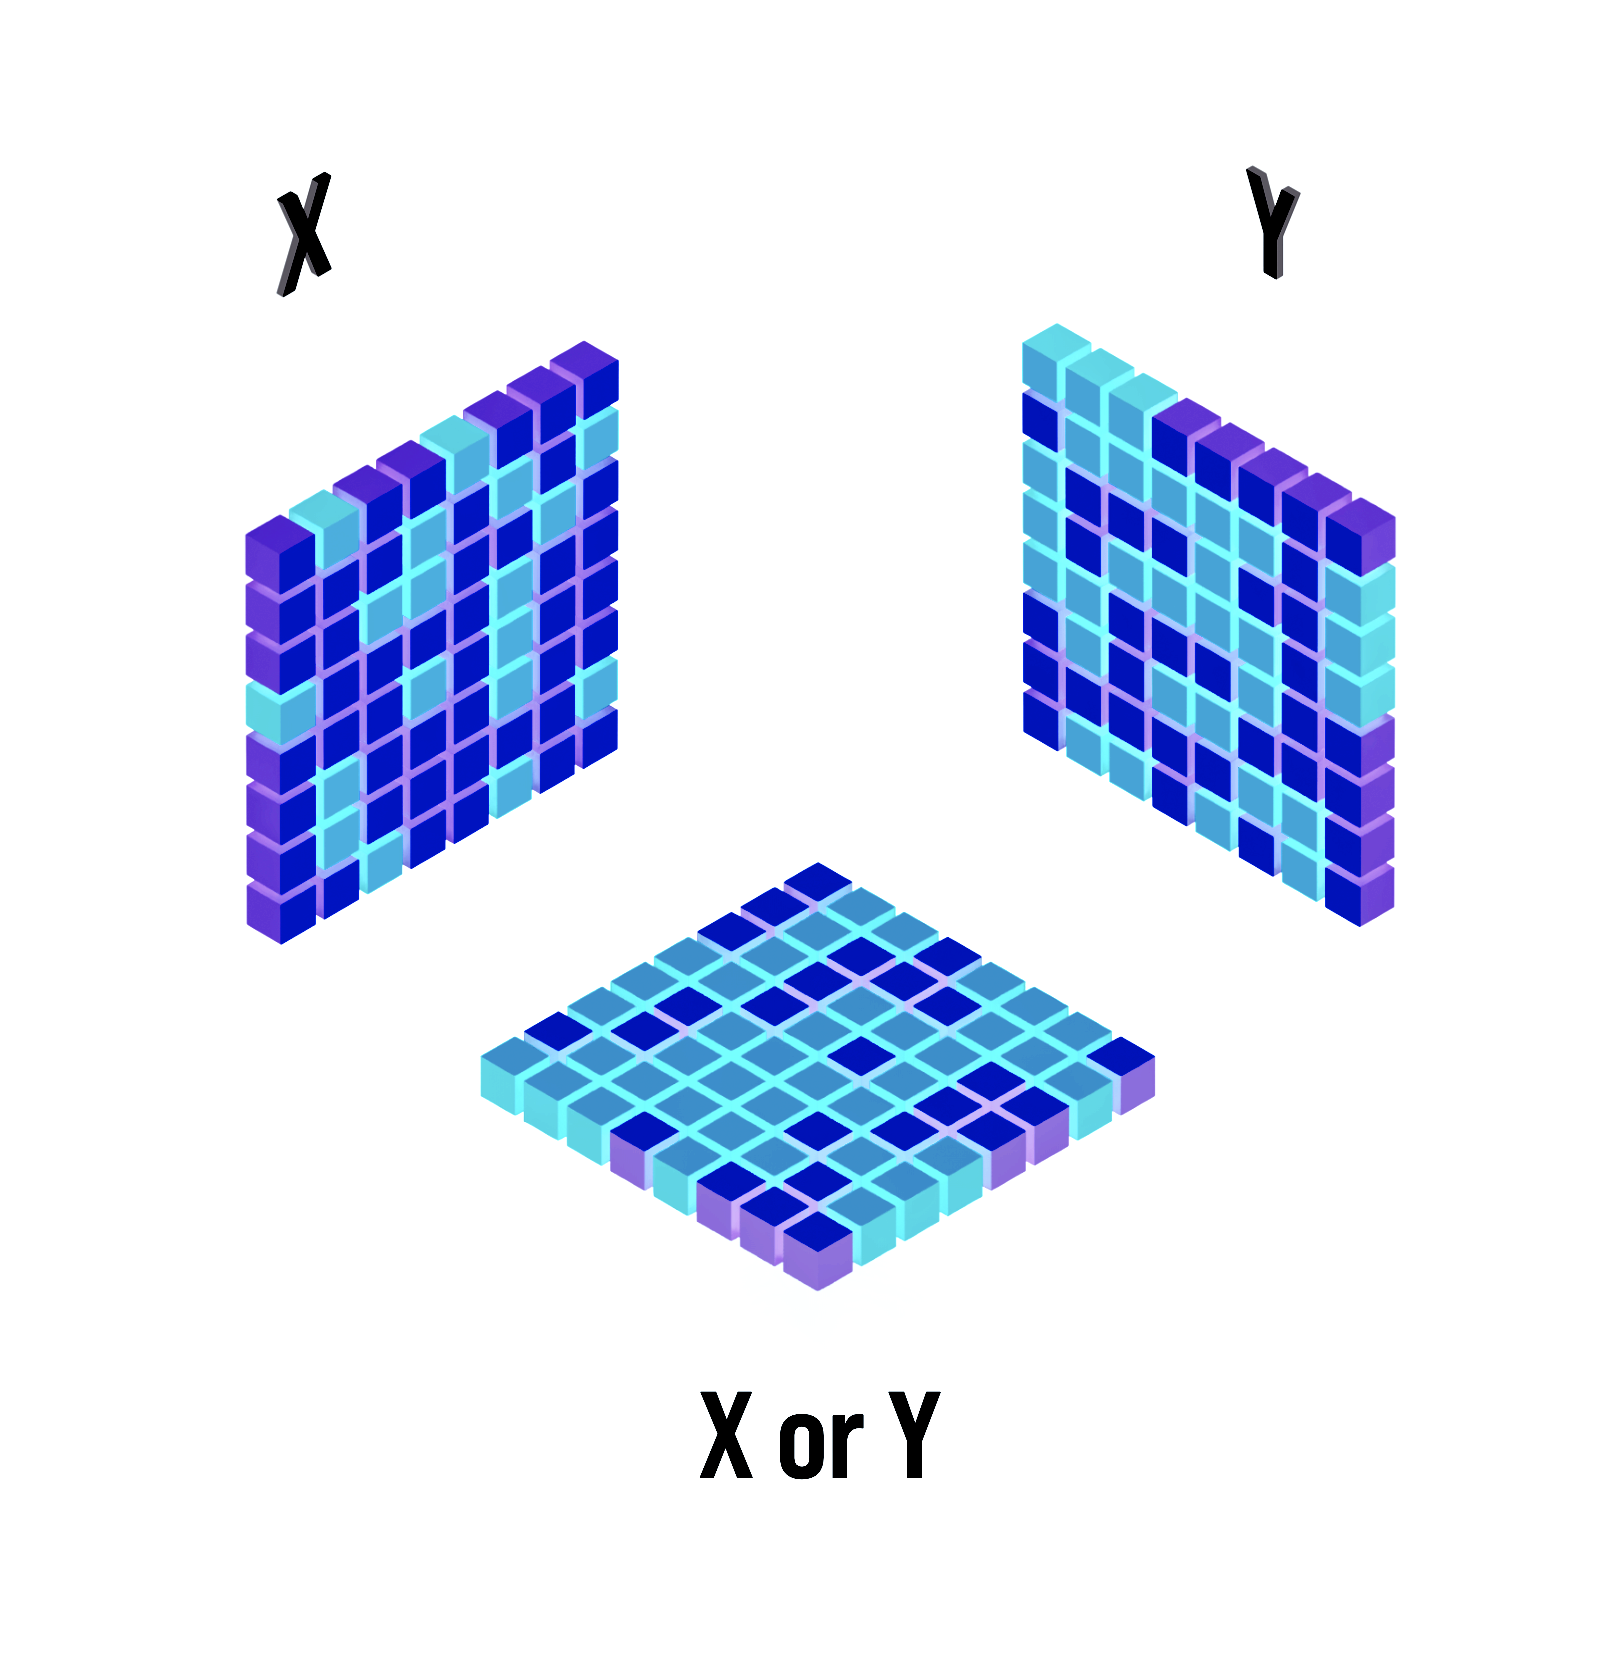
\includegraphics[height=0.7\textheight]{2_framework/research_objective_2_sycl_eval/bitwise_xy_inv.png}
\end{columns}
\end{frame}


% special case for k/n kernels
% ------------ Slide 1a : Original Voting Gate -----------------
\begin{frame}[t]{What is a $k$-of-$n$ (Voting) Gate?}
  \begin{columns}
    % Gate graphic
    \column{0.30\textwidth}
      \centering
    \begin{figure}[h!]
    \tikzset{
    grow'=down,
    level distance=16pt,
    % sibling distance=24pt,
    % sibling distance=8mm/#1,
    level/.style={sibling distance=3pt+44pt/(#1*#1*0.75)},
    edge from parent/.append style={
        draw,
        %thick,
        edge from parent path={
        (\tikzparentnode.west) |- ($(\tikzparentnode.west)!0.5!(\tikzchildnode.east)$) -| (\tikzchildnode.east)
        },
    },
    every node/.append style={
        anchor=center,
        rotate=90,
        draw=black,
        fill=white,
        thick,
        font=\footnotesize\bfseries,
        text centered,
        inner sep=0pt
    },
    var/.style={
        shape=circle,
        minimum height=16pt,
    },
    and/.style={
    and gate US,
    },
  not/.style={
    not gate US,
  },  
  or/.style={
    or gate US,
  },
  vot/.style={
    or gate US,
  }
}
    \centering
    \resizebox{\textwidth}{!}{%
\begin{tikzpicture}[
    circuit logic US,
    tiny circuit symbols,
    level 1/.style={sibling distance=18pt},
    level 2/.style={sibling distance=18pt},
    ]
  \node[or]{\rotatebox{-90}{\tiny{3/5}}}
  % Subset of size 5
  child {
    child { node[var] {\rotatebox{-90}{$X_1$}} }
    child { node[var] {\rotatebox{-90}{$X_2$}} }
    child { node[var] {\rotatebox{-90}{$X_3$}} }
    child { node[var] {\rotatebox{-90}{$X_4$}} }
    child { node[var] {\rotatebox{-90}{$X_5$}} }
  };
\end{tikzpicture}
    }
    \label{fig:example-3of5-voter-tree_no_expansion}
\end{figure}

      \\[-4pt] \scriptsize Example: $k=3$, $n=5$
    % Bullets
    \column{0.70\textwidth}
      \begin{itemize}[<+->]
        \item Outputs 1 iff at least $k$ of $n$ inputs are 1 (majority / threshold logic).
        \item Classic PRA models expand this gate into basic AND/OR primitives --> leads to combinatorial blow-up.
      \end{itemize}
  \end{columns}
\end{frame}

% ------------ Slide 1b : Naïve AND/OR Expansion -----------------
\begin{frame}[t]{Naïve Expansion => Combinatorial Explosion}
  \begin{columns}
    % Left: bullet explanation
    \column{0.35\textwidth}
      \begin{itemize}[<+->]
        \item Expansion = OR of every subset with $k,\dots,n$ true inputs.
        \item For $n=5$, $k=3$: $\binom{5}{3}=10$ conjunction clauses => 26 total gates after binary-tree lowering.
        \item Complexity becomes $\Theta(2^{n}/\sqrt{n})$ at $k\approx n/2$.
      \end{itemize}
    % Right: expanded tree graphic
    \column{0.65\textwidth}
      \centering
      \begin{figure}[h!]
    \tikzset{
    grow'=down,
    level distance=42pt,
    % sibling distance=24pt,
    % sibling distance=8mm/#1,
    level/.style={sibling distance=3pt+44pt/(#1*#1*0.75)},
    edge from parent/.append style={
        draw,
        %thick,
        edge from parent path={
        (\tikzparentnode.west) |- ($(\tikzparentnode.west)!0.5!(\tikzchildnode.east)$) -| (\tikzchildnode.east)
        },
    },
    every node/.append style={
        anchor=center,
        rotate=90,
        draw=black,
        fill=white,
        thick,
        font=\footnotesize\bfseries,
        text centered,
        inner sep=0pt
    },
    var/.style={
        shape=circle,
        minimum height=16pt,
    },
    and/.style={
    and gate US,
    },
  not/.style={
    not gate US,
  },  
  or/.style={
    or gate US,
  },
  vot/.style={
    or gate US,
  }
}
    \centering
    \resizebox{\textwidth}{!}{%
\begin{tikzpicture}[
    circuit logic US,
    tiny circuit symbols,
    level 1/.style={sibling distance=5*18pt},
    level 2/.style={sibling distance=18pt},
    ]
  \node[or]{\rotatebox{-90}{Y}}
  % Subsets of size 3
  child { node[and] {} 
    child { node[var] {\rotatebox{-90}{$X_1$}} }
    child { node[var] {\rotatebox{-90}{$X_2$}} }
    child { node[var] {\rotatebox{-90}{$X_3$}} }
  }
  child { node[and] {} 
    child { node[var] {\rotatebox{-90}{$X_1$}} }
    child { node[var] {\rotatebox{-90}{$X_2$}} }
    child { node[var] {\rotatebox{-90}{$X_4$}} }
  }
  child { node[and] {} 
    child { node[var] {\rotatebox{-90}{$X_1$}} }
    child { node[var] {\rotatebox{-90}{$X_2$}} }
    child { node[var] {\rotatebox{-90}{$X_5$}} }
  }
  child { node[and] {} 
    child { node[var] {\rotatebox{-90}{$X_1$}} }
    child { node[var] {\rotatebox{-90}{$X_3$}} }
    child { node[var] {\rotatebox{-90}{$X_4$}} }
  }
  child { node[and] {} 
    child { node[var] {\rotatebox{-90}{$X_1$}} }
    child { node[var] {\rotatebox{-90}{$X_3$}} }
    child { node[var] {\rotatebox{-90}{$X_5$}} }
  }
  child { node[and] {} 
    child { node[var] {\rotatebox{-90}{$X_1$}} }
    child { node[var] {\rotatebox{-90}{$X_4$}} }
    child { node[var] {\rotatebox{-90}{$X_5$}} }
  }
  child { node[and] {} 
    child { node[var] {\rotatebox{-90}{$X_2$}} }
    child { node[var] {\rotatebox{-90}{$X_3$}} }
    child { node[var] {\rotatebox{-90}{$X_4$}} }
  }
  child { node[and] {} 
    child { node[var] {\rotatebox{-90}{$X_2$}} }
    child { node[var] {\rotatebox{-90}{$X_3$}} }
    child { node[var] {\rotatebox{-90}{$X_5$}} }
  }
  child { node[and] {} 
    child { node[var] {\rotatebox{-90}{$X_2$}} }
    child { node[var] {\rotatebox{-90}{$X_4$}} }
    child { node[var] {\rotatebox{-90}{$X_5$}} }
  }
  child { node[and] {} 
    child { node[var] {\rotatebox{-90}{$X_3$}} }
    child { node[var] {\rotatebox{-90}{$X_4$}} }
    child { node[var] {\rotatebox{-90}{$X_5$}} }
  }
  % Subsets of size 4
  child { node[and] {} 
    child { node[var] {\rotatebox{-90}{$X_1$}} }
    child { node[var] {\rotatebox{-90}{$X_2$}} }
    child { node[var] {\rotatebox{-90}{$X_3$}} }
    child { node[var] {\rotatebox{-90}{$X_4$}} }
  }
  child { node[and] {} 
    child { node[var] {\rotatebox{-90}{$X_1$}} }
    child { node[var] {\rotatebox{-90}{$X_2$}} }
    child { node[var] {\rotatebox{-90}{$X_3$}} }
    child { node[var] {\rotatebox{-90}{$X_5$}} }
  }
  child { node[and] {} 
    child { node[var] {\rotatebox{-90}{$X_1$}} }
    child { node[var] {\rotatebox{-90}{$X_2$}} }
    child { node[var] {\rotatebox{-90}{$X_4$}} }
    child { node[var] {\rotatebox{-90}{$X_5$}} }
  }
  child { node[and] {} 
    child { node[var] {\rotatebox{-90}{$X_1$}} }
    child { node[var] {\rotatebox{-90}{$X_3$}} }
    child { node[var] {\rotatebox{-90}{$X_4$}} }
    child { node[var] {\rotatebox{-90}{$X_5$}} }
  }
  child { node[and] {} 
    child { node[var] {\rotatebox{-90}{$X_2$}} }
    child { node[var] {\rotatebox{-90}{$X_3$}} }
    child { node[var] {\rotatebox{-90}{$X_4$}} }
    child { node[var] {\rotatebox{-90}{$X_5$}} }
  }
  % Subset of size 5
  child { node[and] {} 
    child { node[var] {\rotatebox{-90}{$X_1$}} }
    child { node[var] {\rotatebox{-90}{$X_2$}} }
    child { node[var] {\rotatebox{-90}{$X_3$}} }
    child { node[var] {\rotatebox{-90}{$X_4$}} }
    child { node[var] {\rotatebox{-90}{$X_5$}} }
  };
\end{tikzpicture}
    }
    \label{fig:example-3of5-voter-tree}
\end{figure}

      \scriptsize 3-of-5 gate expanded to AND/OR Sum-of-Products
  \end{columns}
\end{frame}

% ------------ Slide 2 : Hardware-Native Voting Gate ------------
\begin{frame}[t]{Hardware-Native Voting Gate (No Expansion)}
  \begin{columns}
    \column{0.55\textwidth}
      \begin{itemize}[<+->]
        \item Preserve the gate as one vertex; kernel does bit-parallel population count.
        \item Complexity $\mathcal{O}(n)$ integer ops; counter width $\le 8$ bits for PRA fan-ins (256 inputs).
        \item Graph shrinks from $\Theta(2^{n}/\sqrt{n})$ to \textbf{1}. Huge memory & launch savings.
      \end{itemize}
    \column{0.45\textwidth}
      \centering
      \includesvg[height=5cm]{2_framework/research_objective_2_sycl_eval/3_of_5.svg} % placeholder
  \end{columns}
\end{frame}


%% ------------------------------------------------------------------
%% SYCL Execution Model
%% ------------------------------------------------------------------
\subsection{The SYCL Execution Model}
\begin{frame}{SYCL Execution Model in a Nutshell}
      \centering
      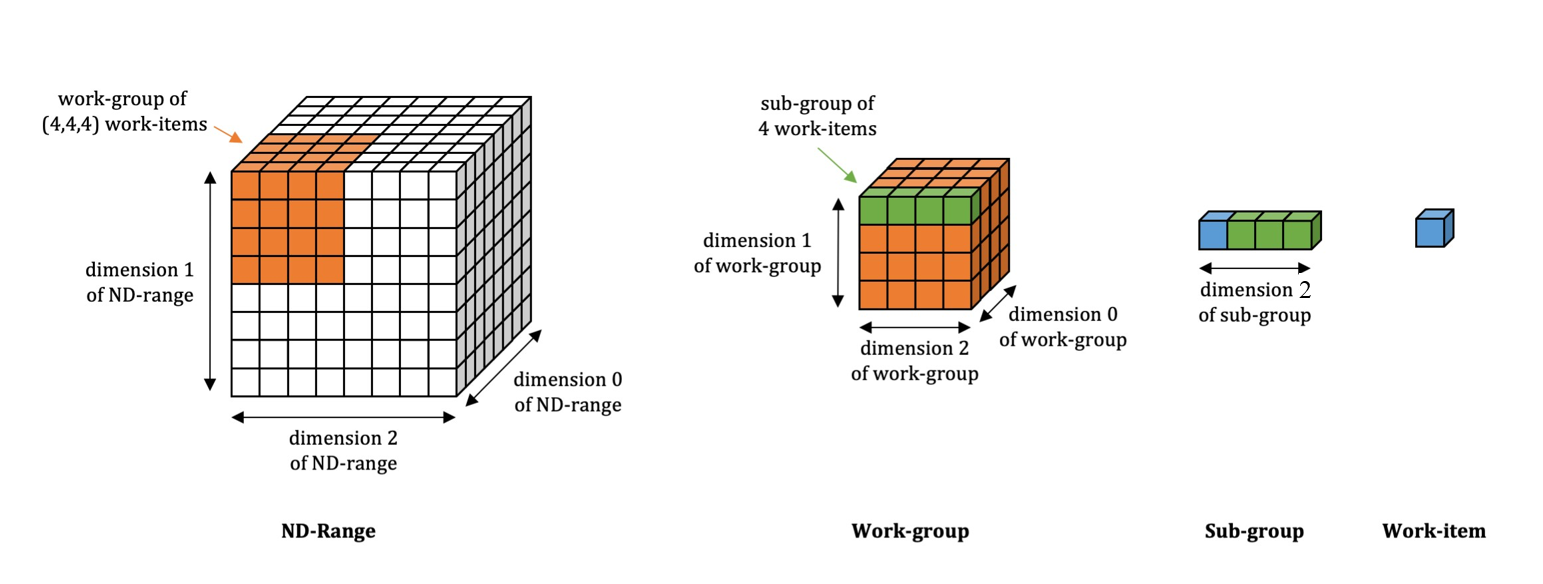
\includegraphics[width=0.9\textwidth]{2_framework/research_objective_2_sycl_eval/sycl.png}\par % Replace with your image file
\end{frame}

%% ------------------------------------------------------------------
%% SYCL Execution Model
%% -----------------------------------------------------------------

\begin{frame}{SYCL Execution Model in a Nutshell}
  \begin{columns}
    \column{0.3\textwidth}
      \tiny
      \begin{description}
        \item[Host] submits \texttt{queue.submit()} with a \texttt{kernel\_name}.
        \item[ND-Range] $\langle\,\text{global}\;3\!\times\!\text{local}\,\rangle$ defines grid.
        \item[Work-Group] maps to CUDA block / OpenCL work-group.
        \item[Sub-Group] (warp/wavefront) gives warp-level shuffle & ballot ops.
        \item[Device USM] used for persistent bit-packed buffers.
      \end{description}
    \column{0.7\textwidth}
      \centering
      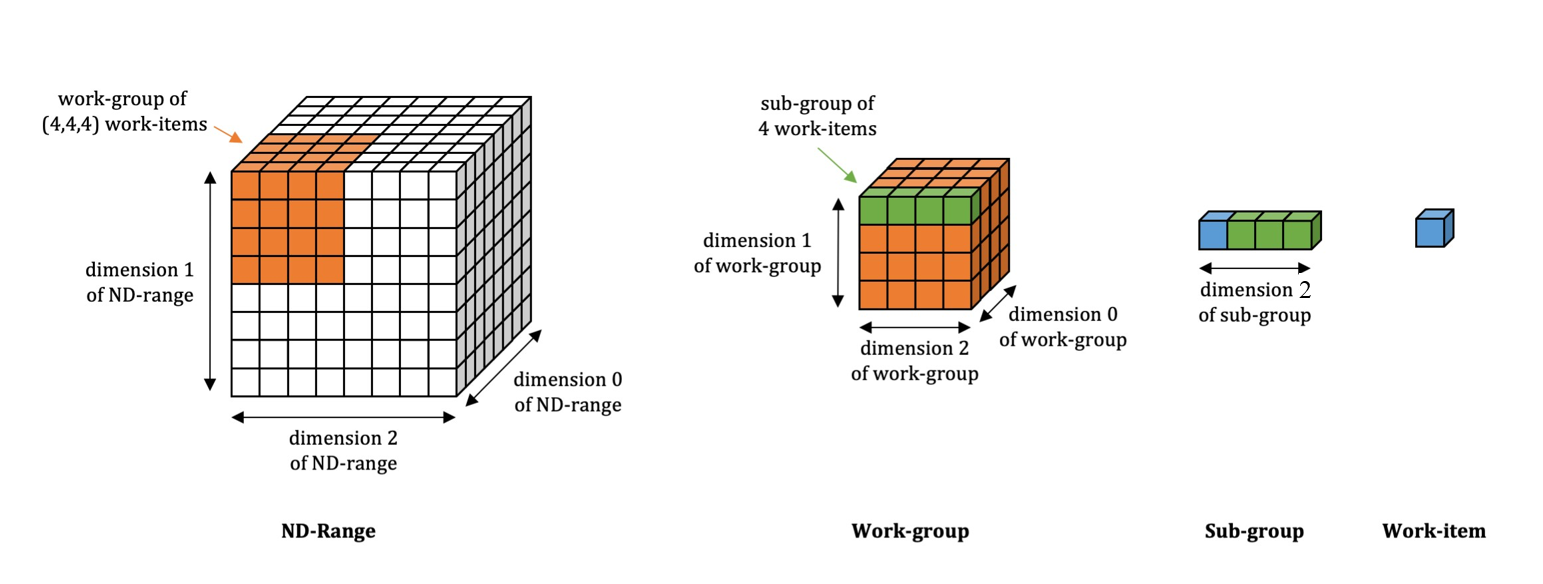
\includegraphics[width=1\textwidth]{2_framework/research_objective_2_sycl_eval/sycl.png}\par % Replace with your image file
  \end{columns}
\end{frame}

%% ------------------------------------------------------------------
%% Mapping PDAG Layers to Kernels
%% ------------------------------------------------------------------
\subsection{Kernel Execution}
\begin{frame}{Mapping PDAG Layers to SYCL Kernels}
    \tiny
  \begin{enumerate}
    \item Topological sort $\Rightarrow$ depth index $d$.
    \item All nodes with depth $d$ share \emph{identical fan-in length}.  \texttt{range<3>} := $(\text{batch},\text{gate},\text{bitpack})$.
    \item One kernel per layer; gate type dispatched via template specialization.
    \item Streams results to next-depth buffer in global memory.
  \end{enumerate}
  \vspace{-42pt}
  \begin{columns}
      \column{0.6\textwidth}
        \centering
      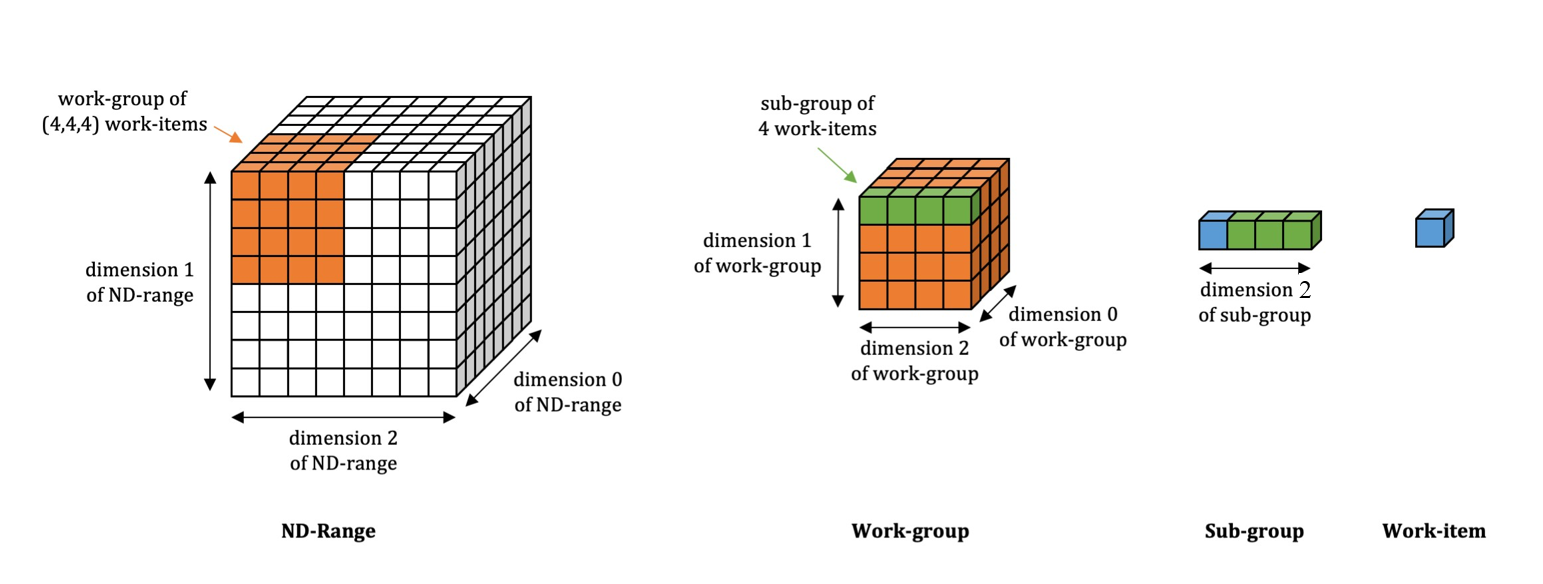
\includegraphics[width=1\textwidth]{2_framework/research_objective_2_sycl_eval/sycl.png}
      \column{0.4\textwidth}
        \centering
        \includesvg[height=0.9\textheight]{1_concepts/dag_pass_2.svg}
  \end{columns}

\end{frame}

\begin{frame}{Eval Query Performance on Generic Backends}
\centering
        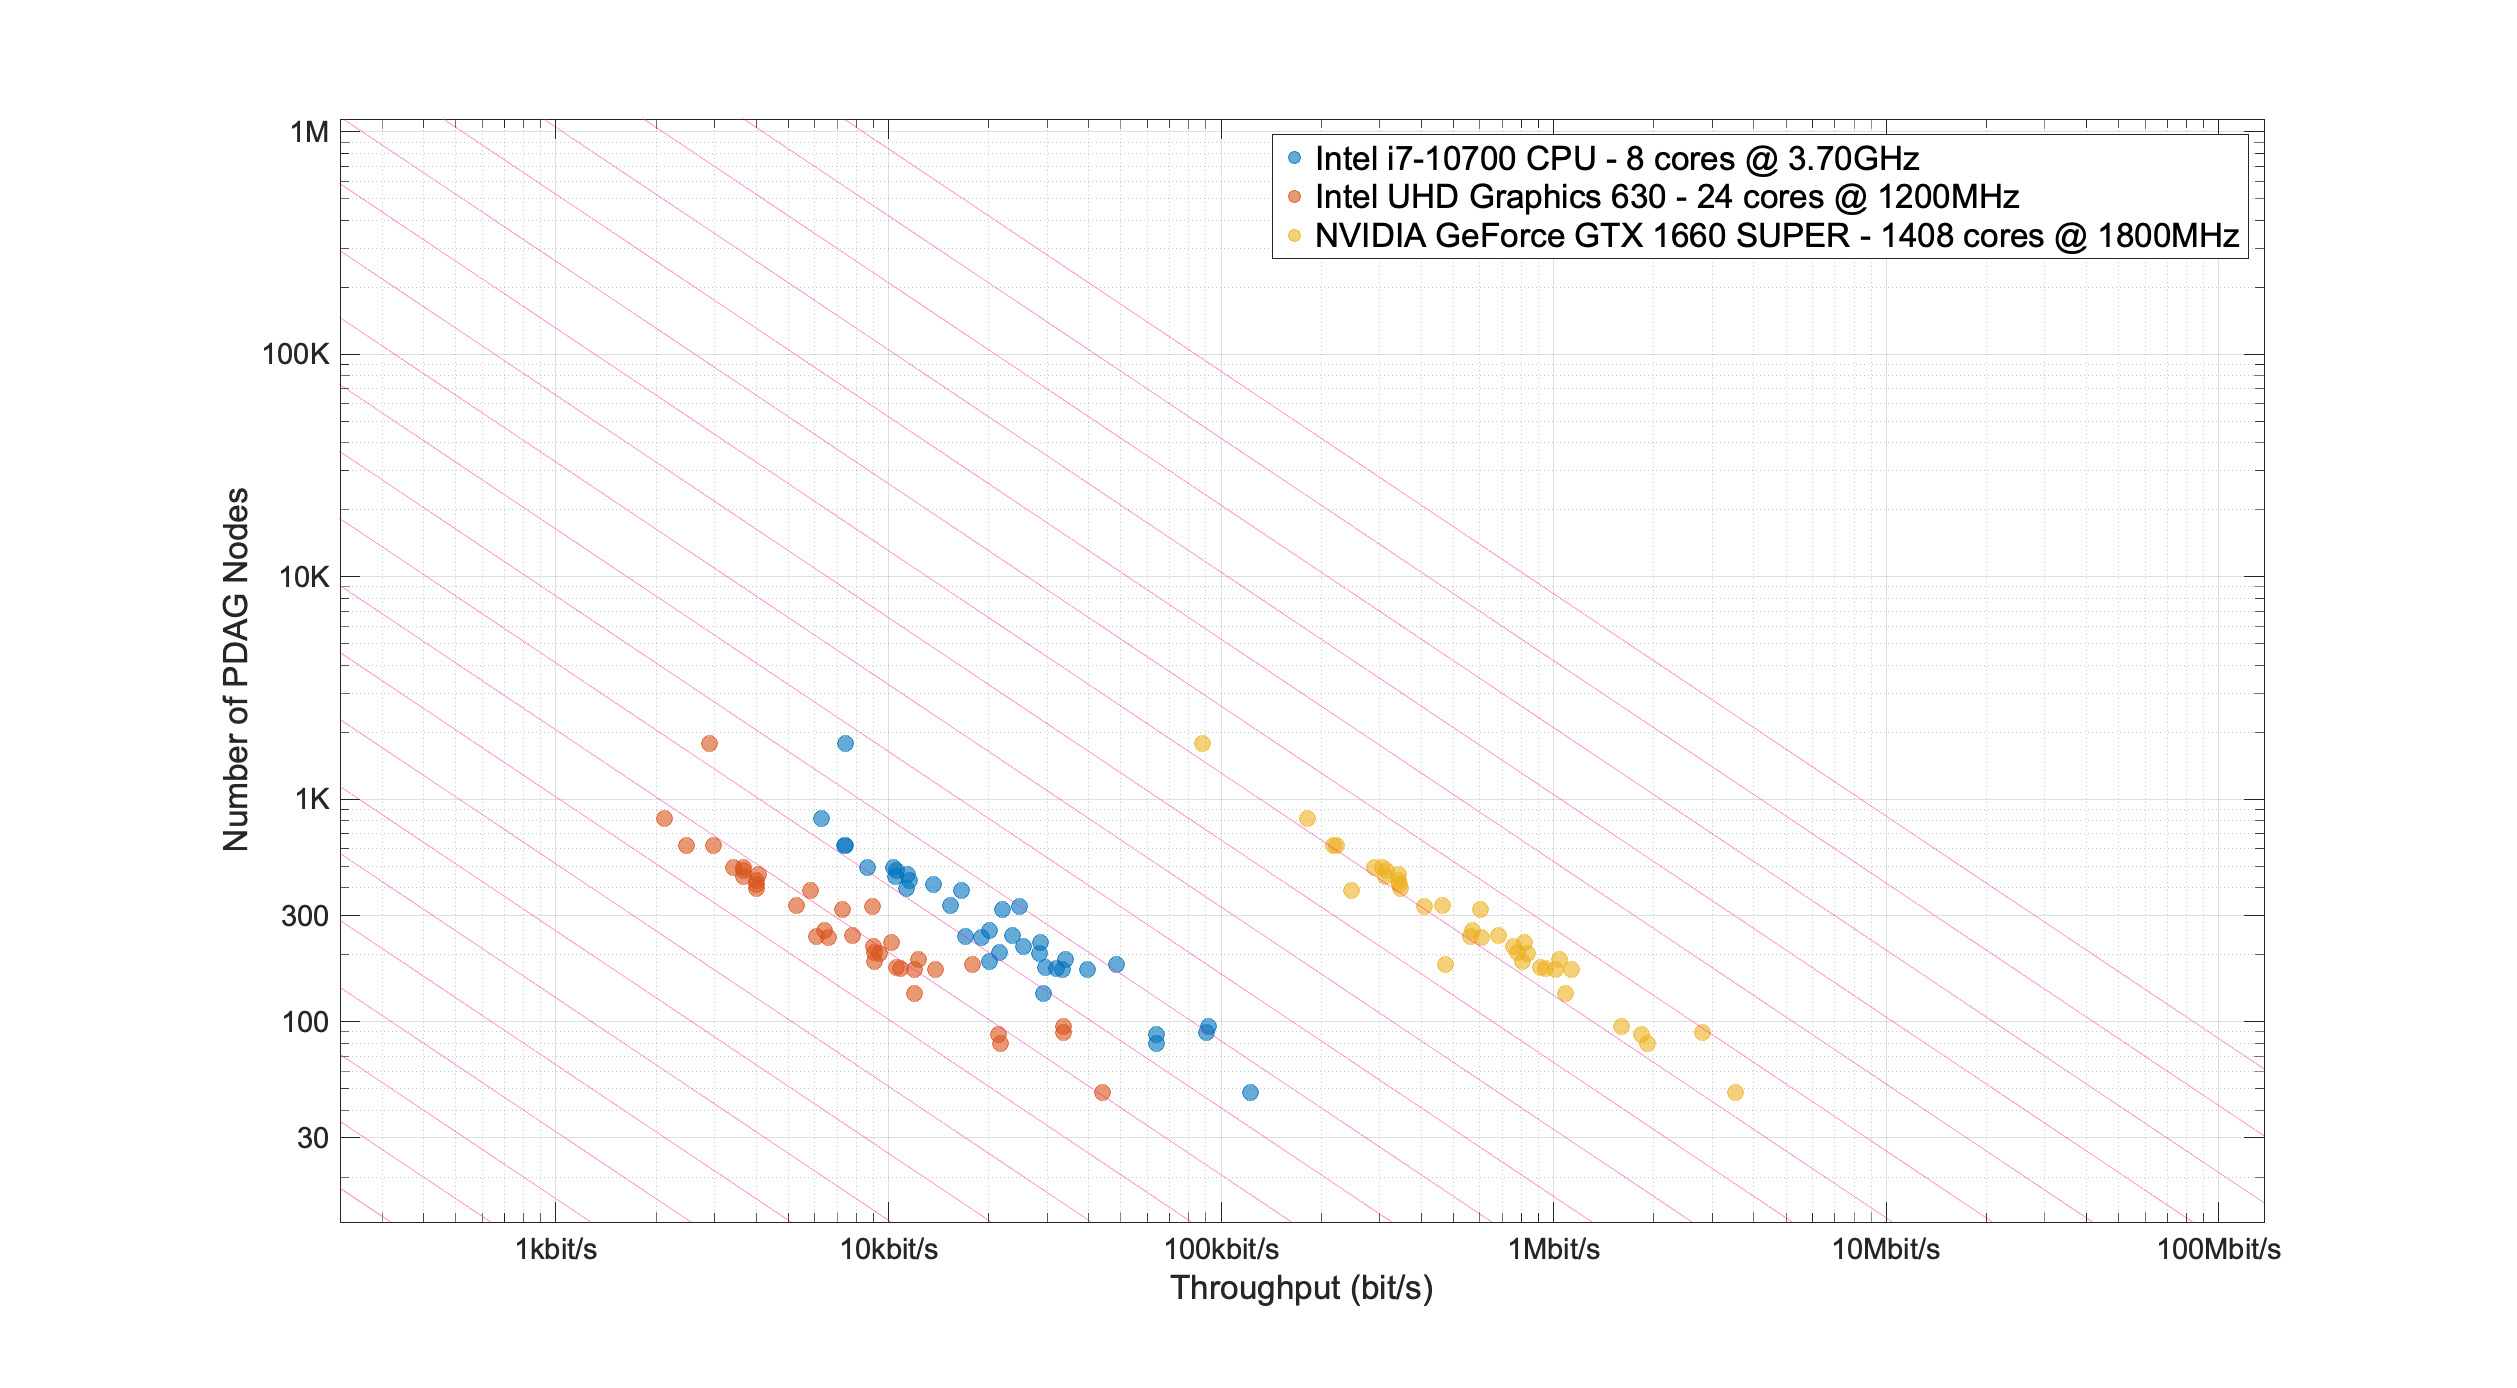
\includegraphics[height=0.9\textheight]{2_framework/research_objective_2_sycl_eval/slides_nodes_vs_throughput.eps}
\end{frame}

%% throughput graph
\begin{frame}{Eval Query Performance on Discrete GPUs}
  \begin{columns}
    \column{0.60\textwidth}
    {
      \begin{itemize}
          \item {Latency: 20-30 $ms$ per layer.}
          \item {Throughput: Graph depth and VRAM bound (see plot).}
          \item {Benchmarked on Nvidia GTX 1660 [6GB].}
          \item {Graph sizes: from $\approx 50$ to $\approx 2000$ nodes.}
          \item {Evals: from 16M to 1B per node per pass.}
      \end{itemize}
      \vspace{10pt}
      \textbf{Q: Are these enough samples to estimate the Expectation Query?}
    }
     \column{0.4\textwidth}
        \centering
        \includesvg[height=0.9\textheight]{1_concepts/mem_allocation_lines_zoom.svg}
  \end{columns}
\end{frame}



